\documentclass[a4paper,10pt,twoside]{article}
%\pagestyle{plain}

\usepackage[spanish]{babel}
\usepackage [latin1]{inputenc}
\usepackage{amsthm}
\usepackage{amsmath}
\usepackage{amssymb}
%\usepackage[lined,spanish,boxed,linesnumbered]{algorithm2e}
\usepackage{algorithm}
\usepackage{algpseudocode}
\usepackage[conEntregas]{caratula}
\usepackage[margin=0.75in]{geometry}
\usepackage{listings}
\lstset{breaklines=true}
\usepackage[usenames,dvipsnames]{xcolor}
\usepackage{hyperref}
\hypersetup{colorlinks=true,linktocpage}

\begin{document}

\titulo{Trabajo Pr\'actico 2}

\fecha{\today}

\materia{Sistemas Operativos}

\integrante{Silvio Vileri\~no}{106/12}{svilerino@gmail.com}
\integrante{Ezequiel Gambaccini}{715/13}{ezequiel.gambaccini@gmail.com}
\integrante{Martin Arjovsky}{683/12}{martinarjovsky@gmail.com}

\maketitle

\tableofcontents

%incluye un abstract de lo que trata el trabajo
\begin{abstract}
INTRO ABSTRACT
\end{abstract}



%contiene la info de que se hizo con servidor_multi
\section{Dise\~no: Modelo propuesto para servidor multihilo}

Se utilizo como base el servidor mono, para realizar el nuevo diseno del servidor multi, que atiende varios clientes de forma concurrente. A continuacion se explica brevemente el funcionamiento del servidor mono y luego se explica como fue implementado el servidor que atiende pedidos concurrentes.

\subsection{Funcionamiento del servidor mono}
El servidor mono atiende un cliente a la vez en base al orden de llegada, y hasta que no termina con el cliente que est\'a atendiendo, no pasa a atender al pr\'oximo.

El protocolo cliente-servidor que se utiliza es el siguiente:
\begin{enumerate}
\item El cliente indica su nombre y posici\'on inicial. Para mantener la simplicidad esta posici\'on no se chequea, por lo que ser\'a el cliente el encargado de enviar una posici\'on v\'alida.
\item El cliente indica el pr\'oximo movimiento, enviando ARRIBA, ABAJO, IZQUIERDA, DERECHA. El servidor recibe el pedido y responde OK u OCUPADO seg\'un corresponda.
\item Las partes repiten este ciclo hasta que el cliente haya salido del lugar. Una vez que esto ocurre, el servidor espera por un rescatista para el alumno y cuando lo obtiene, le coloca la m\'ascara y env\'ia al cliente LIBRE!
\end{enumerate}

Si la conexi\'on se interrumpe en medio de la huida, el servidor da de baja al cliente autom\'aticamente.
Ejemplo:

\begin{figure}[H]
\centering
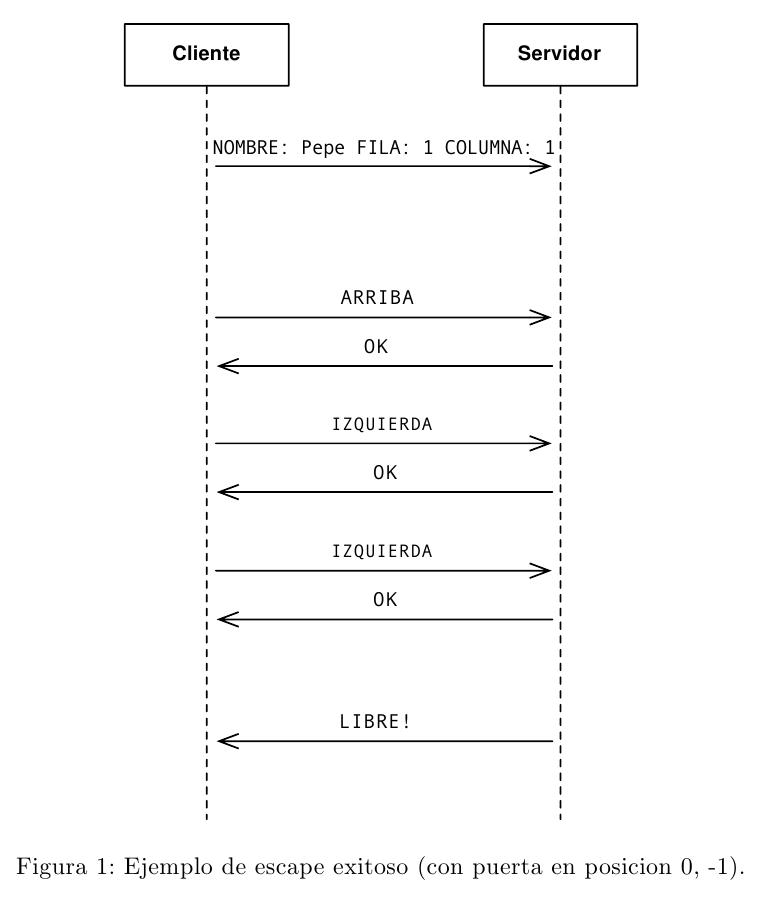
\includegraphics[scale=0.6]{img/prot.jpeg}
\end{figure}

\subsection{Implementaci\'on del servidor multi}

Nuestro servidor multi consiste de un thread principal y un thread worker por cada cliente conectado, separando en hilos diferentes las operaciones que realizaba el servidor mono, como se explica a continuaci\'on:

\begin{itemize}
\item El thread principal se encarga de detectar la conexi\'on de nuevos clientes, tras lo cual crea un worker para que los atienda, si la funcion \verb|pthread_create| devuelve error, se esperan unos segundos y se reintenta la creacion del mismo una cantidad fija de veces antes de ignorar el pedido.
\item El worker se encarga de atender a los clientes usando el protocolo cliente-servidor especificado anteriormente, recibiendo como par\'ametros el socket donde se conect\'o el cliente, y la estructura compartida tipo \verb|t_aula| aula.
\end{itemize}

Para sincronizar los accesos a los diferentes recursos compartidos del aula, prevenir race conditions, se utilizaron diferentes estructuras de sincronizaci\'on del est\'andar pthread, \verb|pthread_mutex_t| y \verb|pthread_cond_t|, en las funciones \verb|t_aula_ingresar|, \verb|t_aula_liberar|, \verb|intentar_moverse|, y \\\verb|atendedor_de_alumno|. La variable de condici\'on solo fue utilizada para la funci\'on \verb|atendedor_de_alumno|.

Una race condition es cuando var\'ia la ejecuci\'on dependiendo del orden de acceso a un recurso compartido, si este orden no es el esperado. Para evitar esto, se fuerza un orden determinado mediante diferentes estructuras de sincronizaci\'on, como mutex y variables de condici\'on.

Un deadlock es la situaci\'on donde 2 threads con 2 recursos tratan de acceder a un recurso que posee el otro, manteniendo el recurso que ya tienen, quedando el sistema bloqueado. Esto en este caso no sucede debido a que solamente se comparte un solo recurso entre todos los threads que es necesario para completar su ejecuci\'on, por lo que no se produce hold & wait, que es lo explicado anteriormente.

Se utilizan en total 3 mutex y 1 variable de condicion:

\begin{itemize}
\item Se utiliza un mutex para sincronizar el acceso a la matriz de posiciones del aula.
\item Se utiliza otro mutex para sincronizar el acceso a la cantidad de personas del aula.
\item Por \'ultimo, se utilizan en conjunto un mutex y una variable de condici\'on para sincronizar el acceso a los rescatistas del aula.
\end{itemize}

Las diferentes funciones especificadas anteriormente acceden a recursos compartidos con todos los clientes, por lo que se usan las estructuras antes especificadas para que el acceso al recurso sea hecho de manera at\'omica y ordenada.

Una consideraci\'on especial que tomamos para nuestro servidor multi fue validar que la posici\'on inicial este dentro del rango de la matriz, y que la celda correspondiente a esta posici\'on tenga lugar disponible para el nuevo cliente. Si no se cumpliera alguna de las condiciones anteriores, se le env\'ia un mensaje de error al cliente, se cierra la conexi\'on y finaliza la ejecuci\'on de ese worker particular. Para realizar esto tambi\'en se tuvo que tener en cuenta posibles race conditions, por lo que se sincronizo el acceso con los mutex especificados anteriormente.

\subsection{Funcionamiento de los threads}

Las operaciones que realiza el hilo principal son las siguientes:

\begin{enumerate}
\item Crear el socket servidor. bindearlo y empezar a escuchar.
\item Inicializar las estructuras de sincronizaci\'on.
\item Quedarse en un loop infinito aceptando conexiones entrantes, creando workers en modo DETACHED para que atiendan las nuevas conexiones realizadas, pasando como par\'ametro el socket de la conexi\'on y un puntero al aula. Se los crea en modo DETACHED ya que no importa cuando terminen ni su valor de retorno, son independientes al thread principal.
\end{enumerate}

Las operaciones que realiza un hilo worker son las siguientes:

\begin{enumerate}
\item Recibir el nombre y posici\'on del cliente.
\item Tratar de hacer entrar al alumno (nuevo cliente), al aula. Si lo logra, se prosigue con la operaci\'on normal, en caso contrario, como se especific\'o anteriormente, se env\'ia un mensaje de error al cliente, se cierra la conexi\'on, y se finaliza la ejecuci\'on de ese worker particular.
\item Luego, el cliente manda una direcci\'on y el servidor le dice si puede avanzar o no. Se repite este ciclo hasta que el cliente sale. Las funciones de acceso al aula son de acceso at\'omico gracias a los mutex.
\item Mediante la combinaci\'on mutex/variable de condici\'on, el worker se queda esperando hasta que la cantidad de rescatistas disponibles sea mayor a 0, para luego marcar que el alumno tiene la mascara puesta.
\item Finalmente, el worker emite un broadcast a la variable de condici\'on para indicar que termin\'o, incrementa en 1 la cantidad de rescatistas, avisa al cliente que es libre, cierra la conexi\'on, y finaliza su ejecuci\'on.
\end{enumerate}

Dado que en la implementacion monothread, podia haber un \'unico cliente moviendose por la matriz, salvo que la cantidad de personas por posicion fuera menor que uno, no hab\'ia problemas de saturaci\'on al momento de entrar. Ahora, dado que puede haber muchos clientes moviendose por la matriz, se debe tener en cuenta la cantidad de personas actualmente en una posicion $(x,y)$ ante un pedido de movimiento o de ingreso al aula. En esta situaci\'on, se debe validar que la posici\'on destino a donde va a terminar el cliente que solicito el pedido, este en rango y ademas que haya lugar para esa persona. Esto provoc\'o tener que crear un nuevo tipo de mensaje de respuesta del servidor (sin modificar el protocolo ya existente) que ante el pedido de ingreso al aula de una posicion $(x,y)$ saturada, se le niegue el ingreso devolviendo dicho nuevo estado \verb|POSICION_LLENA_O_FUERA_DE_RANGO|. Esto no modifica de ninguna forma el protocolo existente, dado que el cliente que vino en el bundle no valida errores. Si el servidor original devolv\'ia errores (el mono devuelve error y el cliente no valida) el cliente no tiene comportamiento definido ante esto. Una forma de solucionar el problema de cambio de protocolo, es definir que \verb|POSICION_LLENA_O_FUERA_DE_RANGO| sea equivalente a \verb|ERROR|, cosa que ya estaba contemplada en el protocolo original presentado.

El tester python otorgado, tampoco validaba si el servidor devolv\'ia \verb|ERROR|, y se limitaba a enviar c\'iclicamente mensajes de forma serial a todos los sockets abiertos. Cuando el servidor devuelve error, cierra el socket y cuando el tester envia datos en el proximo ciclo a un socket cerrado hay un error. Para evitar esto, se validaron las respuestas del servidor, de forma tal que cuando un cliente era liberado/hab\'ia error, se eliminaba del ciclo de proceso de peticiones.

Para testear paralelismo, se corren varios testers de python en paralelo usando bash. En este archivo se pueden encontrar variables de ajuste de parametros tales como cantidad de clientes por thread y cantidad de threads, lo que da una carga del servidor igual a $cantidad\ de\ threads \times cantidad\ de$ $\ clientes\ por\ thread$

%contiene la info de los analisis realizados
\section{Testing: Analisis de escalamiento}
\subsection{Race conditions y Leaks de memoria}
El servidor multi fue testeado para ambas cosas con las herramientas \verb|valgrind --leak-check=full| y \verb|valgrind --tool=helgrind| y se intent\'o realizar una prueba con \verb|thread-sanitizer| de \verb|clang|, pero debido a problemas de instalaci\'on de \verb|clang/compilacion| en \verb|x86|/\verb|x64| no se logr\'o realizar los tests a tiempo.

\subsection{Testing: Analisis de escalabilidad}
A priori existe una cantidad de clientes $k \in \mathbb{N}$ tal que el servidor comienza a tener una ejecucion poco viable, lease consume mucha memoria ram, debido a la creacion excesiva de nuevos hilos, este valor es dificil de determinar dado que si queremos asegurar buen funcionamiento, debemos correr el servidor con valgrind para chequear leaks de memoria y problemas de pthreads y esto produce mucho overhead en el uso de ram del proceso del servidor sobre valgrind, pero a partir de un numero aproximado de 175 clientes concurrentes comienza a haber problemas de conexion, errores de \verb|colabuf| de la biblioteca proporcionada y de lectura-escritura en los sockets. 

\subsubsection{Respecto a cambios en el hardware y la arquitectura fisica del sistema}
Hasta cierto punto, puede ser viable agregar mas memoria ram y tener un servidor totalmente dedicado a atender clientes. El calculo de la RAM asignada al servidor debe hacerse con una estimacion aproximada del peor caso acerca de la carga total del servidor (cantidad de clientes simultaneos + 1), dado que este sera el numero maximo de hilos que puede manejar, habria que calcular en peor caso, cuanta memoria RAM utiliza cada thread(tienen entre otras cosas, pila y registros unicos por thread) y cuanta memoria ram usa el thread principal y el overhead del sistema operativo y la creacion del proceso que encapsula todos los threads.
A partir de que esta solucion no mejore, se puede recurrir a sistemas distribuidos que balanceen la carga de forma mas uniforme y permitan el escalamiento a la cantidad de clientes requerida, un ejemplo seria asignar una porcion de la matriz a cada estacion de trabajo.

\subsubsection{Respecto al software}
Al utilizar threads y no procesos(hijos creados con fork, por ejemplo), se gana en performance dado que el fork es bastante mas costoso que un pthread\_create. Asimismo los cambios de contexto tiene un overhead mucho menor en threads respecto a procesos, aproximadamente de un orden de magnitud teorico. Fueron utilizados en principio por netscape navigator y tuvieron exito dada la ganancia en performance mencionada anteriormente. Como desventaja, todos los threads comparten los mismos datos y es necesario tomar recaudos para la correcta sincronizacion entre ellos. Otro problema es que cualquier libreria que se use debe ser thread-safe.
Como eleccion para maximizar el rendimiento y minimizar el consumo es buena la eleccion de threads sobre procesos como mencionamos anteriormente, pero ademas otra medida podria ser minimizar el uso de variables de stack en los threads, dado que esto aparentemente disminuiria muy poco, pero hay que multiplicarlo por la cantidad de hilos corriendo, puede ser una mejora significativa. Servidores Web como Apache utilizan threads, ver aqui \url{http://httpd.apache.org/docs/2.2/mod/worker.html}, una idea que podriamos tomar de ahi, es hacer uso de un \verb|pool| de threads libres, los cuales sean asignados cuando se registra un pedido, evitando el overhead de la creacion del thread, y reponiendo en el \verb|pool| otro hilo concurrentemente. 

%info acerca del entregable de este trabajo
\section{Ap\'endice: Entregable}
Se entregara tanto el informe como el codigo completos, en un archivo comprimido.
\subsection{Compilaci\'on y ejecuci\'on}
Dado que la \'unica modificaci\'on fue la creacion de un servidor paralelo servidor multi, con solo compilar tipeando \verb|make clean all| se obtendr\'an todos los ejecutables necesarios para llevar a cabo cualquier prueba o ejecuci\'on del sistema. Para ejecutar el servidor se debe tipear \verb|./servidor_multi| y para realizar las pruebas \verb|multi_threaded_tester.sh|. Los par\'ametros modificables que permiten varios tipos de pruebas del servidor se encuentran en \verb|biblioteca.h| y los de testing en \verb|multi_threaded_tester.sh|.


\end{document}

